\documentclass{article}
\usepackage[utf8]{inputenc}

\usepackage[square,numbers]{natbib}
\bibliographystyle{abbrvnat}

\usepackage{amsthm}
\usepackage{amsmath}
\usepackage{hyperref}
\usepackage{caption}
\usepackage{subcaption}
\usepackage{graphicx}

\usepackage[margin=1.2in]{geometry}

\DeclareMathOperator*{\argmax}{arg\,max}
\newcommand{\HRule}{\rule{\linewidth}{0.2mm}}

\begin{document}

\begin{minipage}{\textwidth}
    \begin{center}
        \Large Bayesian Learning\\
        \large Final Report\\
        \HRule\\
        \vspace{0.3cm}
        {\huge \textbf{Bayesian PCA}}\\
        \HRule\\
        \vspace{1em}
            \textbf{Maxence Giraud}\\
            maxence.giraud.etu@univ-lille.fr\\
    \end{center}
\end{minipage}

\begin{abstract}
    In the paper "Bayesian PCA" by Bishop \cite{bishop1999bayesian}, the author describes how one can extend the technique of Principal Component Analysis (PCA) to a Bayesian formulation. In this paper we summarize this new formulation and try to extend it using a Kernel to make a Bayesian Kernel PCA.
\end{abstract}


\section{Introduction}

\subsection{PCA}
We consider a dataset $D$ contained in the matrix $\mathbf{X}$ with its columns representing the features and the rows the data points (so it is an $N \times d$ matrix with $N$ datapoints and $d$ features). For simplicity we will also consider that this data is centered ($\mathbf{x_i} = \mathbf{x_i} - \bar x$).
The conventional PCA starts by computing the sample covariance matrix : 
\begin{equation}
    \mathbf{S} = \dfrac{1}{N} \mathbf{X}^T \mathbf{X} 
    \label{sample_cov}
\end{equation}


We then compute the eigenvectors $\mathbf{u_i}$ and eigenvalues $\lambda_i$ of $\mathbf{S}$ such that : $\mathbf{S}\mathbf{u_i} =\mathbf{S}\lambda_i $.  We only retain the q (the desired dimensionality of the latent space) eigenvectors corresponding to the biggest eigenvalues. And so the new representation of the data is defined using $\mathbf{X_{new}} = \mathbf{U}^T \mathbf{X}$ with $\mathbf{U} = (\mathbf{u_1},...,\mathbf{u_q})$.

\subsection{Probabilistic PCA}

Tipping and Bishop \cite{tipping1999ppca} showed how PCA can be formulated in a probabilistic framework as the maximum likelihood solution of a specific latent variable model.\\
In the first time they introduce a q-dimensionallatent variable $\mathbf{y}$ whose prior distribution is a zero mean Gaussian $p(y) = \mathcal{N}(0,\mathbf{I}_q) $ ($\mathbf{I}_q$ being the q-dimensional identity matrix). And so the observed variable $x$ (we still consider the observation are centered at 0) is defined as a linear transformation (represented by the $d \times q$ matrix $\mathbf{W}$) of $y$ with an additive Gaussian noise ($\epsilon \sim \mathcal{N}(0,\mathbf{I}_d$) )  : $p(\mathbf{x} \mid \mathbf{y}) = \mathbf{W} \mathbf{y} + \epsilon$.\\
The marginal distribution of the observed variable is then given by the convolution of two Gaussians and so is itself Gaussian :

$$p(\mathbf{x})=\int p(\mathbf{x} \mid \mathbf{y}) p(\mathbf{y}) d \mathbf{y}=\mathcal{N}(0, \mathbf{C})$$

with $\mathbf{C} = \mathbf{W} \mathbf{W}^T + \sigma^2 \mathbf{I}_d $. Then we can find the log likelihood of the model given by  :
\begin{equation}
    L\left(\mathbf{W}, \sigma^{2}\right)=-\frac{N}{2}\left\{d \ln (2 \pi)+\ln |\mathbf{C}|+\operatorname{Tr}\left[\mathbf{C}^{-1} \mathbf{S}\right]\right\}
    \label{ll}
\end{equation}

The values of the model's parameters $\mathbf{W}$ and $\sigma$ can be found using multiple methods. We can find an analytical solution by maximizing \ref{ll} or one can use the EM algorithm. We will discuss this second solution more in depth with the Bayesian PCA formulation.

\section{Bayesian PCA}

For the Bayesian PCA we take the same formulation as for the probabilistic PCA on which we are going to add a prior $p(\mathbf{W},\sigma)$ over the parameters of the model, here the likelihood is given by eq \ref{ll} (its logarithm more precisely) and so the posterior $p(\mathbf{W},\sigma\mid D)$ is the product of the two. Then we can obtain the predictive density by marginalizing over the parameters : $p(\mathbf{x} \mid D) = \int \int p(\mathbf{x} \mid \mathbf{W},\sigma) p(\mathbf{x} \mid D) d\mathbf{W} d \sigma$.\\

The author states that the goal of his paper is to automatically find the effective dimensionality of the latent space (which is the number of principal components $q$ in the original PCA formulation), and so to do this he indroduces a hierarchical prior over $\mathbf{W}$ conditionned by a vector $\mathbf{\alpha} = {\alpha_1,...,\alpha_q}$($q$ is set to the maximum possible value $d-1$ by default) that will control this dimensionality.\\
This prior is of the form : 

\begin{equation}
    p(\mathbf{W} \mid \mathbf{\alpha}) = \prod_{i=1}^q (\frac{\alpha_i}{2 \pi})^{d/2} \exp(-\frac{1}{2} \alpha_i \| \mathbf{w}_i\|^2)
    \label{w_prior}
\end{equation}

Here the $\alpha_i$ control the inverse variance of the corresponding $\mathbf{w}_i$ (columns of $\mathbf{W}$) so that if a particular $\alpha_i$ has a posterior distribution concentrated at large values, the related $\mathbf{w}_i$  will tend to be small, and so this component won't be used in the latent space.\\


To use the Bayesian PCA, we should marginalize over the posterior of $\mathbf{W}$ (defined in \ref{w_prior}), but since it is not analytically feasible, the author proposes an alternative approache based on a type-II maximum likelihood using a local Gaussian approximation to a mode of the posterior distribution. \\
We now want to find the location $\mathbf{W_{\text{MP}}}$ of the mode, which can be determined by maximizing the posterior distribution given by :

\begin{equation}
    \ln p(\mathbf{W} \mid D)=L-\frac{1}{2} \sum_{i=1}^{d-1} \alpha_{i}\left\|\mathbf{w}_{i}\right\|^{2}+\text { const }
    \label{posterior}
\end{equation}

with L defined in \ref{ll}. Here the $\alpha_i$ are found through the maximum likelihood estimation, which yields : 
\begin{equation}
    \alpha_i = \frac{d}{\|\mathbf{w}_i\|^2}
    \label{alpha}
\end{equation}

As we recall the $\alpha_i$ control the latent space dimensionality, and so the that vectors $\mathbf{w}_i$ for which there is  insufficient support from the data will be close to 0, and so the corresponding alpha will be driven to infinity.\\

The author then proposes to use the following Expectation-Maximization algorithm (EM) to find $\mathbf{W}_{\text{MP}}$ :

\begin{itemize}
    \item Expectation step : 
\end{itemize}
\begin{equation}
    \begin{aligned}
        \langle\mathbf{Y}\rangle &=\mathbf{M}^{-1} \mathbf{W}^{\mathrm{T}} \mathbf{X} \\
        \langle\mathbf{Y},\mathbf{Y}^T\rangle &=\sigma^{2} \mathbf{M}^{-1}+\langle\mathbf{Y}\rangle \langle\mathbf{Y}\rangle^T
    \end{aligned}
    \label{estep}
\end{equation}

with $\mathbf{M} = \mathbf{W}^T \mathbf{W} + \sigma^2 \mathbf{I}_q$.\\

\emph{N.B. : In his original paper Bishop wrote $\langle\mathbf{Y},\mathbf{Y}^T\rangle$ depending on $\mathbf{M}$ and not $\mathbf{M}^{-1}$, this is a mistake that has been corected in the latter works by Bishop and others.}
\begin{itemize}
    \item Maximization step : 
\end{itemize}

\begin{equation}
    \begin{aligned}
        \widetilde \mathbf{W} &=\mathbf{X} \langle\mathbf{Y}\rangle [\langle\mathbf{Y},\mathbf{Y}^T\rangle + \sigma^2 \mathbf{A}]^{-1} \\
        \tilde{ \sigma^2} &= \frac{1}{N d} \{ \|\mathbf{X}\|^2 -2  \langle\mathbf{Y}^T\rangle \widetilde \mathbf{W}^T \mathbf{X} + \operatorname{Tr}[\langle\mathbf{Y},\mathbf{Y}^T\rangle ] \widetilde \mathbf{W}^T \widetilde \mathbf{W} \}
        \end{aligned}
    \label{mstep}
\end{equation}

with $\mathbf{A}$ a diagonal matrix with the values of the $\alpha_i$ in its diagonal, and as the $\alpha_i$ are computed based on $\mathbf{W}$ they need to be re-evaluated at each step using \ref{alpha}.\\

We can notice that we could use a very similar EM algorithm to solve the probabilistic PCA problem. It can be shown  \cite{tipping1999ppca} that the only modification we would have to make would be to remove the $\sigma^2 \mathbf{A}$ term in the computation of $\widetilde \mathbf{W}$.\\


As we can easily guess, the main contribution of Bayesian PCA is its ability to find automatically the number of effective dimensions $q_{\text{eff}}$. Now an interesting question we could ask ourselves would be how to transpose this paradigm with the Kernel PCA decomposition algorithm.

\section{A Bayesian Kernel PCA}

\subsection{The Kernel PCA and the Kernel Trick}

The PCA allows us to compute a low-dimensional linear embedding of some data, however we may want to be able to also transform our data into a non-linear form. It is where the Kernel PCA comes into play.\\
The original PCA is computed using a sample covariance matrix \ref{sample_cov}, but can also be found by replacing this matrix by the inner product matrix \cite{KevinP.Murphy17} $\mathbf{X} \mathbf{X}^T$ :

$$ S = \frac{1}{N} \mathbf{X}^T \mathbf{H} \mathbf{H} \mathbf{X}, \text{ with }  \mathbf{H} = \mathbf{I}_N -\frac{1}{N} \mathbf{1}_N \mathbf{1}_N^T
$$

Since this covariance Matrix has the same (non zero) eigenvalues as $\frac{1}{N} \mathbf{H}  \mathbf{X}^T \mathbf{X} \mathbf{H}$,by using whats called the Kernel Trick we can replace the inner product by the Kernel $\mathbf{K}$ (we call $\mathbf{K} = \mathbf{X}\mathbf{X}^T$ the gram matrix), this allows us to work with non linear data without having to do the computations in a higher dimensional space.

\subsection{Probabilistic view of the Kernel PCA}


We still assume as with probabilistic PCA that $ \mathbf{X} = \mathbf{W} \mathbf{Y} + \epsilon$ ,  and so we can obtain \cite{pkpca} :

\begin{equation}
    p(\mathbf{X} \mid \mathbf{Y}) = \mathcal{N}(\mathbf{W} \mathbf{Y},N \sigma^2 (\mathbf{I}_N \otimes \mathbf{I}_q ) )  
\end{equation}

In addition, using Bayes’ rule, we can compute the conditional distribution of $\mathbf{Y}$ given $\mathbf{X}$. That is, it follows a multivariate normal distribution:

\begin{equation}
    p(\mathbf{Y} \mid \mathbf{X}) =  \mathcal{N}(\mathbf{M}^{-1} \mathbf{W}^T \mathbf{X}, N \sigma^2 \mathbf{M}^{-1} \otimes \mathbf{I}_N)
\end{equation}

with similarly as classic PCA, $\mathbf{M} = \mathbf{W}^T \mathbf{W} + \sigma^2 \mathbf{I}_q $.\\

We can then formulate the full likelihood of our model :

\begin{equation}
    \begin{aligned}
        L &=  \log p(\mathbf{Y},\mathbf{X})\\
        &=  \log p(\mathbf{X} \mid \mathbf{Y}) + \log p(\mathbf{Y}) \\
        &= - \frac{N}{2}  \log \sigma^2  - \frac{1}{2N} \operatorname{Tr}(\mathbf{Y} \mathbf{Y}^T) -  \frac{1}{N \sigma^2} \operatorname{Tr}((\mathbf{X} - \mathbf{W} \mathbf{Y})(\mathbf{X} - \mathbf{W} \mathbf{Y})^T)
    \end{aligned}
    \label{log_pkpca}
\end{equation}

where we have omitted the terms independent of the model parameters. It is easy to find that $\mathbf{Y}$ and $\mathbf{Y} \mathbf{Y}^T$ are the complete-data sufficient statistics for $\mathbf{W}$ and $\sigma^2$ . \\


We can then a similar EM algorithm as for Probabilistic PCA to find the solution of our problem :

\begin{itemize}
    \item E-step :
\end{itemize}

\begin{equation}
    \begin{aligned}
        \langle \mathbf{Y} \rangle &= \mathbf{M}^{-1} \mathbf{W}^T \mathbf{X} \\
        \langle \mathbf{Y},\mathbf{Y}^T \rangle &= N \sigma^2 \mathbf{M}^{-1} + \mathbf{M}^{-1} \mathbf{W}^T \mathbf{H} \mathbf{K} \mathbf{H} \mathbf{W} \mathbf{M}^{-1} 
    \end{aligned}
    \label{e_step_pkpca}
\end{equation}

\begin{itemize}
    \item M-step : 
\end{itemize}

\begin{equation}
    \begin{aligned}
        \widetilde{ \mathbf{W}} &= \mathbf{X} \langle \mathbf{Y} \rangle  (\langle \mathbf{Y}, \mathbf{Y}^T \rangle)^{-1} \\
        \widetilde{ \sigma^2 } &= \frac{1}{N^2} (\operatorname{Tr}(\mathbf{H} \mathbf{K} \mathbf{H})  + \operatorname{Tr}( \langle \mathbf{Y}, \mathbf{Y}^T \rangle \widetilde \mathbf{W}^T \widetilde \mathbf{W} -2 \operatorname{Tr}(\widetilde{ \mathbf{W}} \langle \mathbf{Y}\rangle \mathbf{X})) 
    \end{aligned}
    \label{m_step_pkpca}
\end{equation}


Substituting $\langle \mathbf{Y} \rangle$ and $\langle \mathbf{Y},\mathbf{Y}^T \rangle$ from the Expectation step \ref{e_step_pkpca} into the Maximization step \ref{m_step_pkpca}, we can combine the two into one :

\begin{equation}
    \begin{aligned}
        \widetilde{ \mathbf{W}} &= \mathbf{H} \mathbf{K} \mathbf{H} \mathbf{W} (N \sigma^2 \mathbf{I}_q + \mathbf{M}^-1 \mathbf{W}^T \mathbf{H} \mathbf{K} \mathbf{H} \mathbf{W})^{-1} \\
        \widetilde{ \sigma^2 } &= \frac{1}{N^2} ( \operatorname{Tr}(\mathbf{H} \mathbf{K} \mathbf{H}) - \mathbf{H} \mathbf{K} \mathbf{H} \mathbf{W} \mathbf{M}^{-1} \widetilde{ \mathbf{W}} )
    \end{aligned}
    \label{em_pkpca}
\end{equation}

with a re-estimation of M at each iteration. \\


\subsection{Introducing a Bayesian Kernel PCA}

For a fully bayesian view of Kernel PCA with the same objective as for the original Bayesian PCA introduced by Bishop, we can follow the same reasonning by putting the same hierarchical prior $p(\mathbf{W} \mid \mathbf{\alpha})$ over $\mathbf{W}$ as in \ref{w_prior}. We then have to maximize the log posterior given by \ref{posterior} with this time L given by \ref{log_pkpca}. This leads to the same re-estimation of the  $\alpha_i$ given in \ref{alpha}.\\
We can then derive a similar EM algorithm to compute the solution : 

\begin{equation}
    \begin{aligned}
        \widetilde{ \mathbf{W}} &= \mathbf{H} \mathbf{K} \mathbf{H} \mathbf{W} (N \sigma^2 \mathbf{A} + \mathbf{M}^-1 \mathbf{W}^T \mathbf{H} \mathbf{K} \mathbf{H} \mathbf{W} )^{-1} \\
        \widetilde{ \sigma^2 } &= \frac{1}{N^2} ( \operatorname{Tr}(\mathbf{H} \mathbf{K} \mathbf{H}) - \mathbf{H} \mathbf{K} \mathbf{H} \mathbf{W} \mathbf{M}^{-1} \widetilde{ \mathbf{W}} )
    \end{aligned}
    \label{em_pkpca}
\end{equation}

with again the diagonal matrix $\mathbf{A}$ with for the diagonal the $\alpha_i$ estimated as before.

\section{Experiments}

We have implementated all the algorithms presented in this paper and are available in the following github repository : \url{https://github.com/MaxenceGiraud/BayesianPCA}. \\

We used this \href{https://archive.ics.uci.edu/ml/datasets/Iris/}{iris dataset} to conduct our experiments. The variability can be captured using only 1 dimension. We found similar results when using both methods to solve the PPCA problem (EM and closed form solution). As for the Bayesian PCA we found that it discovers the  correct effective number of dimension, as we can see by visualization the hinton diagram of the $\mathbf{W}$ matrix in figure \ref{fig:hinton_pca}.\\


\begin{figure}[ht]
    \centering
    \begin{subfigure}{.5\textwidth}
      \centering
      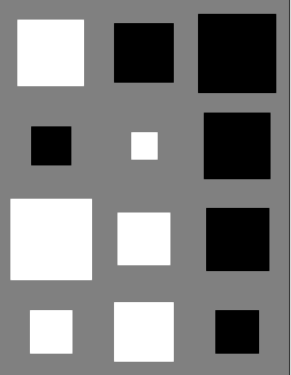
\includegraphics[width=.4\linewidth]{img/hinton_ppca.png}
      \caption{Probabilistic PCA}
      \label{fig:ppca_hinton}
    \end{subfigure}%
    \begin{subfigure}{.5\textwidth}
      \centering
      
\includegraphics[width=.4\linewidth]{img/hinton_bayesian.png}
      \caption{Bayesian PCA}
      \label{fig:bayes_hinton}
    \end{subfigure}
    \caption{Hinton diagrams $\mathbf{W}$ matrix of PPCA and Bayesian PCA}
    \label{fig:hinton_pca}
\end{figure}

We repeated the same experiments with kernel alternative of PCA. We found again similar results for both methods of Probabilistic Kernel PCA  (up to a rotation) and also found that a Linear Kernel would yield similar results as the standard PCA as expected.\\
The Bayesian Kernel PCA also discovers the correct effective number of dimensions, but we can see also see in \ref{fig:pkpca_hinton} that the "simple" probabilistic formulation of the Kernel PCA also shuts off non effective dimensions of the latent space.\\
An interesting follow up to this project would be trying to understand how the probabilistic Kernel PCA shuts off the dimensions and does not show the same behavior as probabilistic PCA.

\begin{figure}[ht]
    \centering
    \begin{subfigure}{.5\textwidth}
      \centering
      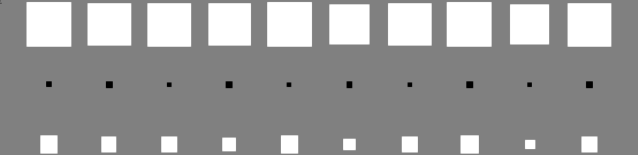
\includegraphics[width=.8\linewidth]{img/hinton_pkpca.png}
      \caption{Probabilistic Kernel PCA}
      \label{fig:pkpca_hinton}
    \end{subfigure}%
    \begin{subfigure}{.5\textwidth}
      \centering
      
\includegraphics[width=.8\linewidth]{img/hinton_bkpca.png}
      \caption{Bayesian Kernel PCA}
      \label{fig:bayesk_hinton}
    \end{subfigure}
    \caption{Hinton diagrams $\mathbf{W}$ matrix of PKPCA and Bayesian Kernel PCA}
    \label{fig:hinton_kpca}
\end{figure}

\section{Conclusion}

In this paper we explored how PCA can be re-formulated in the Bayesian paradigm. The main contribution of this new approach is its ability to approximate the effective number of latent space dimension.\\
We then saw how can the formulation can be combined with the Kernel PCA and how to construct a Bayesian Kernel PCA.\\

We saw some surprising results with Probabilistic Kernel PCA and how even this formulation can be used to approximate the number of effective latent space dimension, this behavior could be investigated in future work.\\

Other continuations of the original paper on Bayesian PCA by Bishop can be made, we can think of properly expressing the optimal dimensionality using conditional probabilities which would be very interesting with the goal of the algorithm.

\bibliography{bayespca}

\end{document}